\documentclass{kjpaper}
\usepackage[authoryear,sort&compress,round]{natbib}
\bibliographystyle{abbrvnat}
\usetikzlibrary{arrows.meta,positioning,calc}
\usepgfplotslibrary{groupplots}
% ---- project macros ----
\newcommand{\sname}{PACT}
% group the size switch so \stdv can be used in running text
\renewcommand{\stdv}[2][\tiny]{{#1\text{$\pm$}#2}}
\title{\sname: A Conflict-Free Lifelong Fleet Manager for Warehouse AMRs and a Controlled Study of Reservation-Aware Pickup Costs}
\correspondingauthor{kangjmo91@gmail.com}
\paperurl{https://github.com/kjungmo/robo-ops}
\author[1]{Jungmo Kang}
\affil[1]{Independent Researcher, Seoul, Republic of Korea}
\keywords{multi-robot task allocation, multi-agent path finding, lifelong pickup and delivery, fleet management, warehouse robotics}
\begin{document}
\begin{abstract}
Fleet managers for warehouse mobile robots must allocate a stream of
pickup-and-delivery tasks, plan collision-free paths for every robot and keep
batteries from running out, all in a loop that never stops. Many fleet
managers connect these problems through free-space distance estimates. Prior
work couples allocation and path finding exactly for one-shot instances, and
approximately in online pickup and delivery by pricing tasks with planned
paths or with the delay that existing reservations impose. In this paper we
introduce \emph{\sname}, an end-to-end lifelong fleet manager for grid
warehouses that uses a cheap member of that family: assignment costs are
arrival times at the pickup of the same windowed space-time A* that plans the
fleet, evaluated against the reservations of the robots that are already
busy, and fed to a Hungarian assignment. A hold cascade, a variant of
existing fail policies that re-plans the robots whose reservations cross a
held cell, keeps prioritized planning conflict-free by construction, and
token-passing endpoint capacities bound dock queues. We prove that
every executed step is vertex- and swap-conflict-free by construction, and
restate the standard optimality of the Hungarian step for its cost matrix;
progress is not guaranteed, and battery
safety holds only under delay bounds that we state but cannot enforce, so we
measure both. We evaluate the whole stack in a seeded discrete-time
simulator with Poisson task streams, loading dwell and an explicit battery
model on four layouts, one of them generated from the zone and dock labels of
an operator-console wireframe and one with one-lane aisles. An independent trajectory
auditor finds no executed conflict in 4{,}740 runs with 60.4 million
robot-steps; with normal batteries no robot depletes and every run delivers
all of its tasks, but with doubled drain the charging policy strands robots
in two thirds of the runs. Without a repair of the reservations that a hold
invalidates, conflicts are executed, and without dynamic priorities the fleet gridlocks. The controlled study of
this pickup-leg coupling, in a loop where dock capacity limits the tasks in
flight, is a negative result that we report as such: greedy, Hungarian,
congestion-proxy and reservation-aware pickup costs stay within 2.9\% of each other
in mean throughput in every one of twelve layout/fleet/load cells, and four
regimes chosen to favour the coupling and committed before their results
(one-lane aisles, hotspot demand, long empty trips, saturated chargers) show
no resolved gain of the reservation-aware cost over greedy assignment in any
regime, and over Hungarian assignment only in the regime in which every method
strands robots; the proxy shows only small effects of either sign outside that
regime.
The study detects no large effect of the cost model but is not an
equivalence test, and it does not cover costs that price the whole trip or
the dock queue. Token passing and token
passing with task swaps deliver 16--66\% less than our loop at its default
dock capacity, mainly because their endpoint rule allows one robot in
flight per dock: with that same limit, token passing with task swaps comes
within 2.5\% of our loop and token passing stays 11--26\% behind. Dock
capacity ($+26$--$29\%$), the planning window
($\pm7\%$) and an optional windowed CBS backend (up to $-8\%$ makespan on small
fleets) are the levers that move the fleet. Code, results and this paper are at
\url{https://github.com/kjungmo/robo-ops}.
\end{abstract}

\maketitle
\section{Introduction}\label{sec:intro}
\begin{figure}[t]
\centering
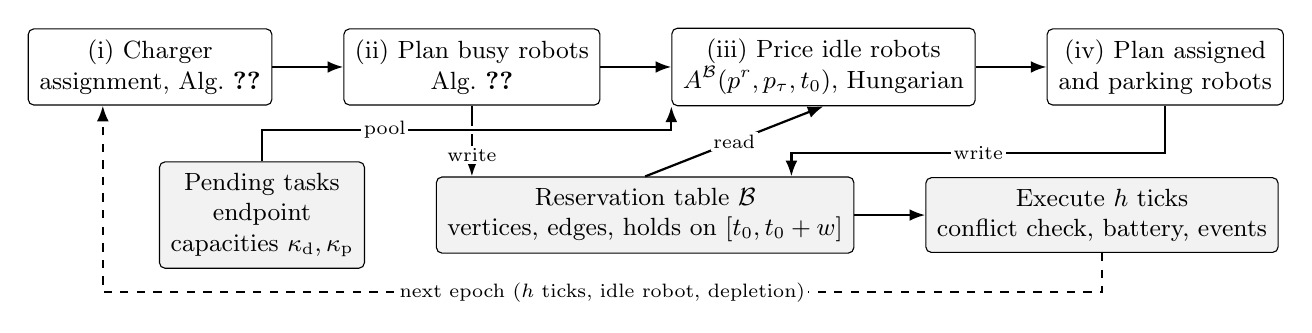
\begin{tikzpicture}[
  font=\small,
  box/.style={draw, rounded corners=2pt, align=center, minimum height=9mm, inner sep=4pt, fill=white},
  stage/.style={box, minimum width=30mm},
  store/.style={box, fill=gray!10, minimum width=26mm},
  arr/.style={-{Latex[length=2mm]}, thick},
  lbl/.style={font=\scriptsize, fill=white, inner sep=1pt}]
  \node[stage] (charge) {(i) Charger\\assignment, Alg.~\ref{alg:charge}};
  \node[stage, right=9mm of charge] (busy) {(ii) Plan busy robots\\Alg.~\ref{alg:pp}};
  \node[stage, right=9mm of busy] (alloc) {(iii) Price idle robots\\$A^{\mathcal{B}}(p^r,p_\tau,t_0)$, Hungarian};
  \node[stage, right=9mm of alloc] (newp) {(iv) Plan assigned\\and parking robots};
  \node[store, below=9mm of busy, xshift=22mm] (table) {Reservation table $\mathcal{B}$\\vertices, edges, holds on $[t_0,t_0+w]$};
  \node[store, left=9mm of table] (tasks) {Pending tasks\\endpoint\\capacities $\kappa_{\mathrm{d}},\kappa_{\mathrm{p}}$};
  \node[store, right=9mm of table] (exec) {Execute $h$ ticks\\conflict check, battery, events};
  \draw[arr] (charge) -- (busy);
  \draw[arr] (busy) -- (alloc);
  \draw[arr] (alloc) -- (newp);
  \draw[arr] (busy.south) -- node[lbl, pos=0.7] {write} (busy.south |- table.north);
  \draw[arr] (table.north) -- node[lbl] {read} (alloc.south);
  \draw[arr] (newp.south) |- node[lbl, pos=0.75] {write} ([xshift=-8mm, yshift=3mm]table.north east) -- ([xshift=-8mm]table.north east);
  \draw[arr, preaction={draw=white, line width=3pt, -}] (tasks.north) |- ++(0,4mm) -| node[lbl, pos=0.15] {pool} (alloc.south west);
  \draw[arr] (table.east) -- (exec.west);
  \draw[arr, dashed] (exec.south) -- ++(0,-5mm) -| ([xshift=-6mm]charge.south) node[lbl, pos=0.25] {next epoch ($h$ ticks, idle robot, depletion)};
\end{tikzpicture}
\caption{\textbf{One replanning epoch of \sname.} Static robots are written as holds and low-charge robots are matched to free charger slots; busy robots, including those just sent to a charger, are then planned into a fresh reservation table; every idle robot is then priced against the candidate pool by running the same windowed space-time A* against the table (a reservation-aware pickup cost), the Hungarian method assigns tasks, and the assigned and parking robots are planned last. A hold cascade (Alg.~\ref{alg:pp}) keeps the table conflict-free whenever a robot cannot find a path.}
\label{fig:overview}
\end{figure}


An operator console for a fleet of autonomous mobile robots (AMRs) shows the
same few things on every screen: which robot is moving where, which task it
carries, how much battery it has and which zone or dock it is heading for.
Behind those screens sits a fleet management system (FMS) that decides all of
it, continuously: new tasks arrive, idle robots must be matched to them,
every robot needs a path that does not collide with any other, and robots
must be sent to chargers before they strand. Each of these problems is well
studied on its own---multi-robot task allocation
\citep{gerkey2004formal,korsah2013comprehensive}, multi-agent path finding
(MAPF) \citep{stern2019mapf,sharon2015cbs} and its lifelong
pickup-and-delivery variant \citep{ma2017lifelong,li2021rhcr}---but a
deployable FMS has to run them together, at every tick, with hard safety
constraints.

The interface between allocation and path finding is where most fleet
managers cut corners. Assignment costs are almost always free-space distances
\citep{ma2017lifelong,liu2019task}, which ignore the traffic that the planner
already knows about; the methods that couple assignment and MAPF exactly
(CBM, \citealp{ma2016optimal}; CBS-TA, \citealp{honig2018cbsta}) solve
one-shot instances and do not transfer to a rolling-horizon loop with
batteries, dwell times and dock queues, and the lifelong scheme that does use
planned arrival times, token passing with task swaps \citep{ma2017lifelong},
applies them greedily, one robot at a time. Whether the cheap decoupling actually
costs anything in a lifelong warehouse setting is, to our knowledge, an open
empirical question; and the planners that make lifelong operation scale
\citep{li2021rhcr} are evaluated without batteries and without dwell times
or capacity limits at the delivery endpoints.

To answer that question with a system rather than a thought experiment, we
introduce \emph{\sname} (Path-Aware Coupled Tasking), an end-to-end,
framework-free lifelong fleet manager for grid warehouses
(\cref{fig:overview}). \sname\ replans the fleet every $h$ ticks over a window
of $w$ ticks, as in RHCR \citep{li2021rhcr}, with windowed space-time A*
\citep{silver2005cooperative} under a reservation table and prioritized
planning \citep{erdmann1987multiple}. Its coupling is deliberately the
cheapest one that uses real plans: the cost of assigning robot $r$ to task
$\tau$ is the arrival time that the same planner reports for $r$'s trip to
the pickup against the reservations of the robots that are already busy, and
the Hungarian method \citep{kuhn1955hungarian} turns those costs into an
optimal assignment. Around the coupling sit the pieces that make a lifelong
loop robust: a hold cascade that converts planner failures into consistent
rests, token-passing endpoint capacities \citep{ma2017lifelong} that keep dock
queues short, a two-threshold charging policy with capacity-constrained slot
assignment, and an optional windowed Conflict-Based Search backend
\citep{sharon2015cbs}.

Our contributions are:
\begin{itemize}
  \item \emph{A tested lifelong FMS stack}: grid map model with benchmark
  layouts (one generated from an operator console's own zone and dock
  vocabulary), Hungarian and greedy allocation, windowed space-time A*,
  prioritized planning with a hold cascade, windowed CBS, charging, and a
  seeded discrete-time simulator; conflict-freeness of every executed step
  and optimality of the assignment step are proved, and a test suite checks the
  Hungarian and CBS implementations against exhaustive search and the planners
  against property tests.
  \item \emph{Path-aware coupled allocation}: assignment costs from
  MAPF-in-the-loop arrival times, with a congestion-proxy middle ground, a
  battery term and candidate pruning, designed so that the coupling adds only
  a bounded number of windowed A* calls per epoch.
  \item \emph{A controlled study of what moves a fleet}: 420 seeded runs on
  three layouts sweep allocation cost model, planner backend, fleet size,
  load regime, window, replanning period, dock capacity and battery
  parameters; a second round of 6{,}180 runs adds a 60-seed safety stress
  test checked by an independent trajectory auditor, an ablation of the hold
  cascade and of the priorities, token-passing baselines and four regimes
  chosen to favour the coupling and committed before their results. Every number traces to a
  committed result file.
\end{itemize}

The study's main result is negative and, we argue, useful: in every one of
twelve layout/fleet/load cells the four allocation cost models---greedy,
Hungarian, congestion proxy and MAPF-in-the-loop---differ by at most 2.9\% in
mean throughput, and 35 of 36 seed-paired 95\% intervals against Hungarian
contain zero (\cref{tab:main,tab:paired}). With five seeds this rules out
differences above about 7\% in the noisiest cell and above about 4\% under the Poisson
load, not small ones. What does move the fleet is elsewhere: raising the
per-dock in-flight capacity from 2 to 3 raises throughput by 26--29\%,
shortening the planning window from 20 to 10 ticks raises it by 7\% while
cutting planner time by $3.3\times$, and windowed CBS reduces makespan by
8\% on small fleets (\cref{tab:ablation,tab:planner}); all three effects lie
outside their seed-paired 95\% intervals. The negative result holds in the
four regimes we chose to favour the coupling (\cref{subsec:coupling}).
Token passing \citep{ma2017lifelong} is 16--66\% slower than our loop at
its default dock capacity, but its endpoint rule allows one robot in flight
per dock; at that capacity our loop and token passing with task swaps are
within $-2.5$ to $+1.6\%$ of each other (\cref{subsec:baselines}), so the
gap measures dock capacity, not our allocation or planner.
Throughout, the executed plans of 60.4 million audited robot-steps contain no
vertex or swap conflict, as the construction guarantees. Progress and charge
are not guaranteed: with normal batteries no robot depletes and every run
delivers all of its tasks, but with doubled drain the charging policy
strands robots once its slots saturate (\cref{subsec:main}), and we prove
only a conditional reserve bound (\cref{prop:charge}). We release the
implementation inside the operator console it was built for, together with
all results.

\section{Related Work}\label{sec:related}

\noindent\textbf{Multi-agent path finding.}
Optimal MAPF on graphs is NP-hard \citep{yu2013structure}; search-based solvers
are surveyed by \citet{felner2017search} and benchmarked under the common
definitions of \citet{stern2019mapf}. Conflict-Based Search (CBS)
\citep{sharon2015cbs} and its improvements
\citep{boyarski2015icbs,li2019symmetry,li2021eecbs} are optimal or
bounded-suboptimal; prioritized planning
\citep{erdmann1987multiple,vandenberg2005prioritized,cap2015prioritized} with a
space-time reservation table \citep{silver2005cooperative} is incomplete but
fast and remains the workhorse of deployed fleets. PIBT
\citep{okumura2019pibt,okumura2022pibt} replaces long-horizon paths with
one-step priority inheritance. \sname\ uses windowed prioritized planning as
its default planner, offers windowed CBS as an optional backend, and adds a
hold cascade that turns planner failures into consistent (conflict-free) rests.

\noindent\textbf{Lifelong pickup-and-delivery.}
Warehouse fleets never solve a one-shot instance: tasks arrive continuously
\citep{wurman2008coordinating}. \citet{ma2017lifelong} formalised
multi-agent pickup and delivery (MAPD), introduced well-formed instances and
the token-passing (TP) scheme, in which a robot only takes a task whose pickup
and delivery are not the endpoint of another robot's path; its variant with
task swaps (TPTS) lets a robot take over an assigned task whose pickup it
reaches earlier than the current assignee, which already couples allocation
to planned arrival times, greedily and one robot at a time.
\citet{ma2019lifelong} added kinematic constraints
and \citet{liu2019task} studied task sequencing. RHCR \citep{li2021rhcr}
showed that replanning every $h$ steps over a window of $w$ steps scales to
hundreds of robots. \sname\ adopts the RHCR execution model and TP-style
endpoint reservation, and evaluates them together with an explicit battery
model, which the cited works abstract away.

\noindent\textbf{Task allocation and its coupling with path finding.}
Assignment problems are classically solved by the Hungarian method
\citep{kuhn1955hungarian,munkres1957algorithms,jonker1987shortest} or by
auctions \citep{bertsekas1988auction}; taxonomies of multi-robot task
allocation are given by \citet{gerkey2004formal} and
\citet{korsah2013comprehensive}. Coupling assignment with MAPF has been done
optimally for teams of interchangeable agents (CBM, \citealp{ma2016optimal})
and for agents with individual sets of admissible goals (CBS-TA,
\citealp{honig2018cbsta}), at a cost that limits these methods to one-shot
instances. \sname\ instead couples the two approximately in the lifelong
loop: assignment costs are arrival times of windowed space-time A* against
the live reservation table, solved jointly for all idle robots by the
Hungarian method, which prices in the traffic that already exists but not the
interactions among the robots being assigned. None of these ingredients is new
on its own; the contribution is their combination with batteries and dock
capacities in one loop, and the controlled measurement of what the coupling
buys.

\section{\sname: A Coupled Lifelong Fleet Manager}\label{sec:method}

\sname\ runs a rolling-horizon loop (\cref{fig:overview}): every replanning
epoch it (i) re-plans the robots that already have goals, (ii) sends
low-charge robots to free charger slots, (iii) prices every idle robot against
the pending tasks and solves an assignment problem, and (iv) plans the newly
assigned robots into the same reservation table. The coupling lives in step
(iii): assignment costs are not free-space distances but arrival times
computed by the same windowed planner against the reservations written in
step (i). We first fix the model (\cref{subsec:model}), then describe the
planning layer (\cref{subsec:planning}), the charging policy
(\cref{subsec:charging}) and the coupled allocation (\cref{subsec:alloc}).

\subsection{Modelling the fleet: lifelong MAPD with battery constraints}\label{subsec:model}

\noindent\textbf{Workspace.}
The workspace is a 4-connected grid graph $G=(V,E)$ with obstacle cells
removed. Four endpoint classes mirror the operator console's vocabulary:
pickup points $\mathcal{P}\subset V$ on shelf lines, delivery docks
$\mathcal{D}\subset V$, charger slots $\mathcal{C}\subset V$ grouped into
stations, and home bays $\mathcal{H}\subset V$, one per robot. Every dock,
slot and bay is a dead-end pocket off a corridor, so an instance is
well-formed in the sense of \citet{ma2017lifelong}: a robot resting on a
non-task endpoint never blocks a path between two other endpoints.
Distances $d(u,v)$ are exact shortest-path lengths on $G$, computed by
breadth-first search from each endpoint and cached.

\noindent\textbf{Robots and tasks.}
A fleet $\mathcal{R}=\{1,\dots,n\}$ of robots moves synchronously in discrete
time $t\in\mathbb{N}$; at every tick a robot either moves to a 4-neighbour or
waits. Robot $r$ has position $p_t^r\in V$, state of charge
$s_t^r\in[0,1]$, and home bay $h^r\in\mathcal{H}$. Tasks arrive as a stream
$\mathcal{T}=\{\tau_k\}$, $\tau_k=(a_k, p_k, d_k)$ with arrival time $a_k$,
pickup $p_k\in\mathcal{P}$ and dock $d_k\in\mathcal{D}$; a robot that reaches
$p_k$ loads for $\delta$ ticks, drives to $d_k$ and unloads for $\delta$
ticks, which completes the task at time $c_k$.

\noindent\textbf{Battery.}
Charge decreases by $\beta_{\mathrm{m}}$ per move and $\beta_{\mathrm{w}}$ per
wait, and increases by $\gamma$ per tick while a robot rests on a charger
slot; a robot with $s^r_t\le 0$ is depleted and becomes a permanent
obstacle. The charging policy is a two-threshold hysteresis
$(\theta_{\mathrm{lo}},\theta_{\mathrm{hi}})$, \cref{subsec:charging}.

\noindent\textbf{Conflicts.}
Two robots conflict when they occupy the same cell at the same tick (vertex
conflict) or traverse the same edge in opposite directions during the same
tick (swap conflict); following a robot into the cell it just left is
allowed, as in the standard MAPF definitions of \citet{stern2019mapf}.

\noindent\textbf{Objective.}
Given the stream $\mathcal{T}$, the fleet manager chooses, at every tick, an
assignment of idle robots to pending tasks, a charging decision and one action
per robot, so as to minimise the mean service time of the delivered tasks
\begin{equation}\label{eq:objective}
  J \;=\; \frac{1}{|\mathcal{T}|}\sum_{\tau_k\in\mathcal{T}} \bigl(c_k - a_k\bigr)
  \quad\text{subject to}\quad
  \text{no conflicts},\;\; s^r_t>0\;\;\forall r,t,
\end{equation}
and we also report throughput $|\mathcal{T}|/T_{\mathrm{mk}}$, where the
makespan $T_{\mathrm{mk}}=\max_k c_k$. For a finite stream throughput is the
inverse makespan, a different objective from mean service time that can rank
schedules differently, so we report both. Optimising \cref{eq:objective} exactly is intractable even
without batteries \citep{yu2013structure}; \sname\ is a rolling-horizon
heuristic. It enforces the conflict constraint by construction
(\cref{prop:pp,cor:exec}); the charge constraint is only guarded by a
heuristic feasibility test (\cref{eq:feasible}), and progress (absence of
deadlock and livelock) is not guaranteed. Both are measured in
\cref{sec:exp}.

\subsection{Planning under reservations: windowed space-time A* with a hold cascade}\label{subsec:planning}

\noindent\textbf{Reservation table.}
A reservation table $\mathcal{B}$ stores, for an epoch starting at $t_0$ with
horizon $t_0+w$, the vertex reservations $(v,t)$ and edge reservations
$(u,v,t)$ of every planned robot, plus \emph{holds} $(v,t_{\mathrm{h}})$
meaning ``occupied from $t_{\mathrm{h}}$ until the horizon''. A path whose
last cell is reached at $t_{\mathrm{e}}\le t_0+w$ ends with a hold, so a
robot that arrives early is a static obstacle for the rest of the window.
The table answers three queries: $\mathrm{free}(v,t)$,
$\mathrm{free}(u\!\to\!v,t)$ (false iff the reverse edge is reserved at $t$)
and $\mathrm{goalfree}(v,t)$ (true iff $v$ is free for all
$t'\in[t,t_0+w]$ and not held).

\noindent\textbf{Windowed space-time A*.}
Each robot plans on the time-expanded graph
$V\times\{t_0,\dots,t_0+w\}$ with the exact distance $d(\cdot,g)$ as
heuristic (\cref{alg:astar}). A state $(g,t)$ is a goal only if
$\mathrm{goalfree}(g,t)$; a state at the horizon is closed with cost
$t-t_0+d(v,g)$ and completed with a deterministic shortest path, because no
reservation exists beyond the horizon. The returned cost is the arrival time
\begin{equation}\label{eq:arrival}
  A^{\mathcal{B}}(p,g,t_0) \;=\; \min\{\,t - t_0 : (g,t)\ \text{reachable under }\mathcal{B},\ \mathrm{goalfree}(g,t)\,\},
\end{equation}
the per-agent cost of sum-of-costs MAPF restricted to the window. Since
$d(\cdot,g)$ is consistent, the first goal state popped is optimal, and the
search is bounded by $|V|(w+1)$ expansions.

\begin{algorithm}[t]
\caption{Windowed space-time A* (one robot)}\label{alg:astar}
\KwIn{start $p$, goal $g$, epoch start $t_0$, window $w$, reservations $\mathcal{B}$, distances $d(\cdot,g)$}
\KwOut{path $\pi=(\pi_0=p,\pi_1,\dots)$ and arrival time, or \textsc{fail}}
$\mathit{open}\gets\{(p,t_0)\}$ with $f=d(p,g)$; $\mathit{closed}\gets\emptyset$\;
\While{$\mathit{open}\neq\emptyset$}{
  pop $(v,t)$ with minimal $f$ (ties: larger $g$-value, then FIFO)\;
  \lIf{$(v,t)\in\mathit{closed}$}{\textbf{continue}}
  add $(v,t)$ to $\mathit{closed}$\;
  \lIf{$v=g$ \KwSty{and} $\mathrm{goalfree}(g,t)$}{\Return path to $(v,t)$, cost $t-t_0$}
  \lIf{$t=t_0+w$}{\Return path to $(v,t)$ followed by a shortest path $v\!\leadsto\! g$, cost $t-t_0+d(v,g)$}
  \ForEach{$v'\in\{v\}\cup N(v)$}{
    \If{$\mathrm{free}(v',t+1)$ \KwSty{and} $(v'=v$ \KwSty{or} $\mathrm{free}(v\!\to\!v',t))$}{
      push $(v',t+1)$ with $f=(t+1-t_0)+d(v',g)$\;
    }
  }
}
\Return \textsc{fail}\;
\end{algorithm}

\noindent\textbf{Prioritized planning with a hold cascade.}
Robots are planned one after another in priority order
(\cref{alg:pp}); each path is written into $\mathcal{B}$ before the next
robot plans. Prioritized planning is incomplete: a robot may find no path
within the window. Instead of leaving such a robot unplanned, \sname\ makes it
\emph{hold} its current cell for the whole window, and re-plans every robot
whose reservation crosses that cell---including robots planned in an earlier
group of the same epoch. Holds only accumulate within an epoch, so the cascade
terminates, and at termination every path is consistent with every
reservation:

\begin{proposition}[Conflict-freeness of an epoch]\label{prop:pp}
Let all robots occupy distinct cells at $t_0$, and let every entry of
$\mathcal{B}$ at the call belong either to an external robot in
$\mathcal{X}$ or to a static robot holding its own current cell. If the
entries of $\mathcal{B}$ are pairwise conflict-free when \cref{alg:pp} is
called, then after it returns the set of paths in $\mathcal{B}$ is vertex-
and swap-conflict-free on $[t_0,t_0+w]$, and \cref{alg:pp} calls the
low-level planner at most $N(N+1)/2\le|\mathcal{R}|(|\mathcal{R}|+1)/2$
times, where $N=m+|\mathcal{X}|$.
\end{proposition}
\begin{proof}
\emph{Invariant.} We show that no two entries of $\mathcal{B}$ conflict at
any moment. A path is inserted only when \cref{alg:astar} returned it under
the current $\mathcal{B}$: every vertex $(\pi_k,t_0+k)$ passed
$\mathrm{free}$, every move passed the swap query, and, if the path reaches
its goal inside the window, the hold at its last cell passed
$\mathrm{goalfree}$, so no existing entry occupies that cell later in the
window (a path that reaches the horizon first is stored only up to the
horizon, without a hold, and its unconstrained tail is never executed); entries inserted afterwards respect the hold because
$\mathrm{free}$ checks holds. A hold for a failed robot $r$ is written at
$p^r$ from $t_0$ on. No static robot and no held robot occupies $p^r$ (their
cells are their own, and start cells are distinct), and by assumption every
other entry belongs to a robot in $\mathcal{X}$ or in the input list; all of
those that visit $p^r$ at some $t\in[t_0,t_0+w]$ form $\mathcal{V}$ and are
removed before the hold is written. A hold never moves, so it cannot take
part in a swap conflict. Removing entries cannot create a conflict, so the
invariant holds at termination.

\emph{Call bound.} A robot is popped once initially if it is in the input
list ($m$ calls) and once each time it is re-queued. Re-queuing happens only
when a hold is created; a held robot is never re-queued (it is excluded from
$\mathcal{V}$) and so fails at most once, hence at most $N$ holds are
created. When the $k$-th hold is created, $|\mathcal{K}|=k$ and
$\mathcal{V}$ contains only robots outside $\mathcal{K}$, so
$|\mathcal{V}|\le N-k$. The number of calls is therefore at most
$m+\sum_{k=1}^{N}(N-k)\le N+N(N-1)/2=N(N+1)/2$.
\end{proof}

The assumption on $\mathcal{B}$ is what the epoch
(\cref{alg:pact}) maintains: static robots are written as holds on their own
cells, group~1 is planned into a table that contains only those holds, and
group~2 is planned with group~1 as $\mathcal{X}$. The optional CBS backend
(below) only inserts paths that are conflict-free with each other and with
$\mathcal{B}$ inside the window, which preserves the invariant, and the
robots it wrote into $\mathcal{B}$ are added to $\mathcal{X}$ of the
subsequent call of \cref{alg:pp} for the rest of the group. Neither the proposition nor its corollary says anything about
progress: a robot may hold for several epochs.

\begin{corollary}[Conflict-free execution]\label{cor:exec}
If $h\le w$, every step executed by the simulator is vertex- and
swap-conflict-free.
\end{corollary}
\begin{proof}
Every robot executes the path it has in the current table: a planned path,
or a hold on its own cell for static robots, and a robot whose path has ended
rests on its last cell, which that path holds. Epochs start at least every
$h$ ticks, so the step from $t$ to $t+1$ executed after an epoch at $t_0$
satisfies $t+1\le t_0+h\le t_0+w$ and lies inside the window in which the
table is conflict-free by \cref{prop:pp}. Between epochs the table changes
only by single-robot re-plans (below): the robot's old entry is removed, and
the new one is either a path returned by \cref{alg:astar} under the table or,
if that fails, a hold on the cell the robot stands on, which its old entry
held from the current tick on, so no other entry uses it. A depleted robot
stops, and an epoch starts before the next step is executed.
\end{proof}

\begin{algorithm}[t]
\caption{Prioritized planning with hold cascade}\label{alg:pp}
\KwIn{ordered robots $(r_1,\dots,r_m)$ with starts and goals, external robots $\mathcal{X}$ already in $\mathcal{B}$, epoch $t_0$}
\KwOut{paths for $r_1,\dots,r_m$ (and re-planned members of $\mathcal{X}$), held set $\mathcal{K}$}
$Q\gets(r_1,\dots,r_m)$; $\mathcal{K}\gets\emptyset$\;
\While{$Q\neq\emptyset$}{
  $r\gets$ pop front of $Q$\;
  $\pi\gets$ \textsc{A*}$(p^r,g^r,t_0,w,\mathcal{B})$ \tcp*{\cref{alg:astar}}
  \If{$\pi=$ \textsc{fail}}{
    $\pi\gets(p^r)$; $\mathcal{K}\gets\mathcal{K}\cup\{r\}$ \tcp*{hold current cell}
    $\mathcal{V}\gets\{\,r'\notin\mathcal{K} : r'$ reserved $(p^r,t)$ in $\mathcal{B}$ for some $t\in[t_0,t_0+w]\,\}$\;
    remove the reservations of every $r'\in\mathcal{V}$ from $\mathcal{B}$\;
    push $\mathcal{V}$ (in priority order) to the front of $Q$\;
  }
  write $\pi$ into $\mathcal{B}$ (with a hold at its last cell if it ends before the horizon)\;
}
\end{algorithm}

\noindent\textbf{Priorities and groups.}
An epoch plans two groups. Group~1 contains the busy robots (driving to a
pickup, a dock or a charger) together with parking robots that either stand
on a busy robot's goal or failed to plan in the previous epoch; group~2
contains the robots assigned in this epoch and the remaining parking robots.
Within a group, robots standing on another robot's goal come first, then
robots held last epoch, then carrying, then collecting, then charging-bound,
then parking robots, ties by id. Planning a held robot first is what evacuates
a robot boxed in on the single access cell of a corner dock; without it the
queue for that dock and the evacuating robot wait for each other
(\cref{sec:disc}). Robots that are charging, loading, unloading, depleted or
idle at home are static and are written as holds before group~1.

\noindent\textbf{Windowed CBS.}
As an optional backend, a group is planned jointly by Conflict-Based Search
\citep{sharon2015cbs} whose low level is \cref{alg:astar} under the union of
$\mathcal{B}$ and the node's constraints, and whose high level only resolves
conflicts inside the window (\cref{alg:cbs}). Two robots that share a goal
are not a valid one-shot instance; the lower-priority one is deferred to
\cref{alg:pp}, as are robots without an individually feasible path and the
whole group when the constraint tree exceeds a node budget.

\begin{algorithm}[t]
\caption{Windowed CBS for one group (high level)}\label{alg:cbs}
\KwIn{robots $\mathcal{A}$ with distinct goals, base reservations $\mathcal{B}$, epoch $t_0$, window $w$, node budget $N_{\max}$}
\KwOut{conflict-free paths on $[t_0,t_0+w]$ with minimal sum of arrival times, or \textsc{fail}}
root: $\mathcal{C}_r\gets\emptyset$, $\pi_r\gets$ \textsc{A*} under $\mathcal{B}\cup\mathcal{C}_r$ for each $r\in\mathcal{A}$\;
\lIf{some $\pi_r=$ \textsc{fail}}{\Return \textsc{fail}}
$\mathit{open}\gets\{\text{root}\}$\;
\While{$\mathit{open}\neq\emptyset$}{
  $\nu\gets$ node with minimal $\sum_r\mathrm{cost}(\pi_r)$ (ties: fewer conflicts, then FIFO)\;
  $\kappa\gets$ earliest conflict of $\nu$ on $[t_0,t_0+w]$\;
  \lIf{$\kappa=\emptyset$}{\Return paths of $\nu$}
  \lIf{$|\text{generated}|\ge N_{\max}$}{\Return \textsc{fail}}
  \ForEach{robot $r\in\kappa$}{
    child $\nu'\gets\nu$ with $\mathcal{C}_r$ extended by the vertex $(v,t)$ or edge $(u\!\to\!v,t)$ of $\kappa$\;
    re-plan $\pi_r$ under $\mathcal{B}\cup\mathcal{C}_r$; \lIf{feasible}{add $\nu'$ to $\mathit{open}$}
  }
}
\Return \textsc{fail}\;
\end{algorithm}

\noindent\textbf{Execution.}
Every tick each robot executes the next action of its path; a robot that
reaches the end of its path at its goal (and only then---a plan may pass
through the goal earlier while the goal is temporarily held) transitions
(pickup $\to$ loading, dock $\to$ unloading, slot $\to$ charging, bay $\to$
idle) and is immediately re-planned alone against the live table when it
gets a new goal; this re-plan keeps the table conflict-free
(\cref{cor:exec}). A new epoch starts every $h\le w$ ticks and whenever a
robot becomes idle while tasks are pending or a robot depletes. Independently
of the reservation table, the simulator compares the cells of all robots
before and after every executed step and counts vertex and swap conflicts;
this check tests the implementation against \cref{cor:exec}, and over all runs
in \cref{sec:exp} the count is zero.

\subsection{Charging: threshold policy with capacity-constrained slot assignment}\label{subsec:charging}

A robot with $s^r_t<\theta_{\mathrm{lo}}$ that is idle or parking must charge
before it accepts work; it leaves the slot when
$s^r_t\ge\theta_{\mathrm{hi}}$. Free slots are those neither occupied nor
already claimed by a robot en route, so a station with $k$ slots serves at
most $k$ robots at a time. Robots needing charge and free slots are matched
by the Hungarian method on $d(p^r,\sigma)$ (\cref{alg:charge}); a robot for
which no slot is free waits at its bay and is retried next epoch. A task
feasibility test guards against stranding: robot $r$ may take task $\tau$
only if
\begin{equation}\label{eq:feasible}
  s^r_t \;\ge\; \beta_{\mathrm{m}}\bigl(\hat a(r,\tau) + d(p_\tau,d_\tau) + \min_{\sigma\in\mathcal{C}} d(d_\tau,\sigma)\bigr) + \rho,
\end{equation}
where $\hat a$ is the estimated time to the pickup used by the allocation
(\cref{subsec:alloc}) and $\rho$ a reserve margin. The test is a heuristic,
not a guarantee: it budgets free-space moves only and leaves waits, detours,
dwell and queueing for a charger slot to the margin $\rho$, and a robot that
depletes nevertheless becomes a permanent obstacle. With
\cref{eq:feasible} and $\theta_{\mathrm{lo}}$ above the energy of the longest
bay-to-slot trip, no depletion occurred in any run of \cref{sec:exp}.

\begin{algorithm}[t]
\caption{Charger assignment (one epoch)}\label{alg:charge}
\KwIn{robots $\mathcal{N}=\{r : s^r_t<\theta_{\mathrm{lo}},\ r$ idle or parking$\}$, free slots $\mathcal{F}\subseteq\mathcal{C}$}
\lIf{$\mathcal{N}=\emptyset$ \KwSty{or} $\mathcal{F}=\emptyset$}{\Return}
$M\gets$ \textsc{Hungarian}$\bigl([\,d(p^r,\sigma)\,]_{r\in\mathcal{N},\sigma\in\mathcal{F}}\bigr)$\;
\ForEach{$(r,\sigma)\in M$}{claim $\sigma$ for $r$; goal of $r\gets\sigma$; status of $r\gets$ charging-bound\;}
\end{algorithm}

\subsection{Allocating tasks: assignment costs from MAPF-in-the-loop}\label{subsec:alloc}

\noindent\textbf{Candidate pool.}
Pending tasks are kept in arrival order. Following token passing
\citep{ma2017lifelong}, a task enters the candidate pool only while its dock
has fewer than $\kappa_{\mathrm{d}}$ robots in flight (assigned and not yet
delivered) and its pickup fewer than $\kappa_{\mathrm{p}}$; the pool holds
the oldest $\max(2m,8)$ such tasks for $m$ eligible robots. This endpoint
reservation is what keeps dock queues short enough for \cref{alg:pp} to
resolve (\cref{subsec:ablation}).

\noindent\textbf{Cost.}
For eligible robot $r$ and pool task $\tau$ the cost is
\begin{equation}\label{eq:cost}
  c(r,\tau) \;=\; \hat a(r,\tau)\,\bigl(1 + w_{\mathrm{b}}\,(1-s^r_t)\bigr),
\qquad
  \hat a(r,\tau) =
  \begin{cases}
    d(p^r,p_\tau) & \text{static (greedy, Hungarian)}\\[2pt]
    d(p^r,p_\tau) + w_{\mathrm{c}}\,\chi_{\mathcal{B}}(p^r\!\leadsto\!p_\tau) & \text{congestion proxy}\\[2pt]
    A^{\mathcal{B}}(p^r,p_\tau,t_0) & \text{path-aware (\sname)}
  \end{cases}
\end{equation}
with $c(r,\tau)=\infty$ when \cref{eq:feasible} fails. The battery factor
makes a low-charge robot look farther, so long trips go to well-charged
robots. The congestion proxy counts, along the free-space shortest path, the
cells reserved by other robots at the time the robot would traverse them
(held cells count $w_{\mathrm{h}}$); the path-aware cost is the arrival time
\cref{eq:arrival} of \cref{alg:astar} against the table that already contains
group~1. Costs are computed for the $K$ nearest pool tasks of each robot
(static distance), other pairs are infeasible.

\noindent\textbf{Assignment.}
The cost matrix is solved by the Hungarian method
\citep{kuhn1955hungarian,munkres1957algorithms} in the
shortest-augmenting-path form of \citet{jonker1987shortest}, applied to the
rectangular matrix, with infeasible
pairs priced above the sum of all finite costs; or, for the greedy baseline,
by repeatedly committing the cheapest remaining pair.

\begin{proposition}[Optimality of the assignment step]\label{prop:hungarian}
For a cost matrix $C\in(\mathbb{R}_{\ge0}\cup\{\infty\})^{m\times k}$, the
Hungarian step returns a matching that, among all matchings of maximum
cardinality over finite entries, minimises total cost; it runs in
$O(\min(m,k)^2\max(m,k))$ time.
\end{proposition}
\begin{proof}
Assume $m\le k$ (otherwise the implementation solves the transpose). Replace
$\infty$ by any $\Lambda>S=\sum_{ij:C_{ij}<\infty}C_{ij}$ (the implementation
uses $S+10^6$); the algorithm returns a minimum-cost matching that covers
every row. Such a matching $M$ with $\ell(M)$ $\Lambda$-entries costs
$\ell(M)\Lambda+F(M)$ with finite part $0\le F(M)\le S<\Lambda$, so a
minimiser first minimises $\ell$ and then $F$. Let $\nu$ be the maximum
cardinality of a matching of finite entries. Any such matching extends to a
row-covering matching because $m\le k$, and the added pairs are all
$\Lambda$-entries (a finite one would give a larger finite matching), so
$\min\ell=m-\nu$ and every maximum finite matching $M'$ appears, extended,
with cost $(m-\nu)\Lambda+F(M')$. Dropping the $\Lambda$-pairs of the
minimiser therefore leaves a maximum-cardinality finite matching of minimum
finite cost. Each of the $m$ rows is inserted by one shortest-augmenting-path
phase with potentials \citep{jonker1987shortest} of $O(mk)$ time, which gives
$O(m^2k)$.
\end{proof}

\begin{algorithm}[t]
\caption{\sname\ epoch (rolling horizon)}\label{alg:pact}
\KwIn{tick $t_0$, robots $\mathcal{R}$, pending tasks, window $w$}
$\mathcal{B}\gets$ empty table on $[t_0,t_0+w]$; release finished chargers; idle robots off their bay become parking\;
write holds for static robots (charging, loading, unloading, depleted, idle at bay)\;
\textsc{ChargerAssignment} (\cref{alg:charge})\;
group~1 $\gets$ busy robots $\cup$ parking robots on a busy goal or held last epoch; \textsc{PP}(group~1, $\mathcal{B}$) (\cref{alg:pp})\;
$\mathcal{E}\gets$ idle/parking robots not in group~1 with $s^r_t\ge\theta_{\mathrm{lo}}$; remove their holds from $\mathcal{B}$\;
build pool with endpoint capacities $\kappa_{\mathrm{d}},\kappa_{\mathrm{p}}$; $C_{r\tau}\gets c(r,\tau)$ by \cref{eq:cost} for $K$ candidates per $r\in\mathcal{E}$\;
$M\gets$ \textsc{Hungarian}$(C)$; assign $(r,\tau)\in M$: goal of $r\gets p_\tau$\;
unassigned $r\in\mathcal{E}$: goal of $r\gets h^r$ (parking)\;
group~2 $\gets$ newly assigned $\cup$ parking robots not in group~1; \textsc{PP}(group~2, $\mathcal{B}$, external = group~1)\;
\end{algorithm}

\noindent\textbf{Complexity.}
Let $|V|$ be the number of free cells. One epoch costs
$O\bigl(|\mathcal{R}|^2\,|V|\,w\bigr)$ for planning (\cref{prop:pp}, each
call bounded by $|V|(w+1)$ expansions; in practice the cascade is rare and
the cost is linear in $|\mathcal{R}|$), plus $O(mK\,|V|\,w)$ for path-aware
pricing and $O(m^2\,|\mathcal{T}_{\mathrm{pool}}|)$ for the assignment. The
static and proxy variants replace the pricing term by $O(mK)$ table look-ups
(distances are cached), which is the entire runtime overhead of the coupling;
\cref{subsec:main} reports it as planner milliseconds per simulated tick.

\section{Experiments}\label{sec:exp}

We ask three questions. (Q1) Is the stack correct and stable in lifelong
operation---no conflicts, no depletions, no deadlocks---across layouts, fleet
sizes and load regimes? (Q2) Does coupling allocation to the planner through
path-aware costs improve throughput or service time over static costs?
(Q3) Which of the remaining design choices (planner backend, window,
replanning period, endpoint capacity, battery term) matter, and what do they
cost in planner time?

\subsection{Experimental Setup}\label{subsec:setup}

\noindent\textbf{Layouts.}
\emph{warehouse} ($52\times19$, 715 free cells) has four blocks of five
10-cell shelf lines with 2-wide aisles, 100 pickup points, 9 docks, 4 charger
stations of 2 slots and 48 home bays. \emph{console} ($36\times25$, 658 free
cells) is generated from the zone/line/dock counts that appear in the
operator console's wireframe labels (zones A--D with 3, 3, 2 and 4 shelf
lines; two named shipping docks, modelled as bays of three delivery cells), 84
pickups, 6 docks, 3 stations, 32 bays. \emph{small} ($16\times10$, 104 free
cells) is an open floor with 4 pickups, 2 docks, 2 slots and 8 bays used for
the planner comparison. \Cref{tab:layouts} in the appendix lists all counts.

\noindent\textbf{Tasks and load.}
Each run delivers 200 tasks (100 on \emph{small}) whose pickup and dock are
sampled uniformly. Two load regimes are used: a Poisson stream of
$\lambda=0.15$ tasks per tick, which is below the capacity of fleets of 16 or
more robots and saturates a fleet of 8, and \emph{batch}, which releases all
tasks at $t=0$ and measures pure throughput. Loading and unloading dwell is
$\delta=2$ ticks. Initial charge is uniform in $[0.5,1.0]$, except in the
battery stress where it is uniform in $[0.2,0.4]$ so that every robot has to
charge during the run. All parameters are listed in \cref{tab:params}.

\noindent\textbf{Methods.}
Four allocation cost models share the same planner, charging policy and
endpoint capacities: \emph{Greedy} (cheapest pair first, static distance),
\emph{Hungarian} (optimal assignment, static distance), \emph{Proxy}
(Hungarian on distance plus reservation-table congestion, \cref{eq:cost}) and
\emph{\sname} (Hungarian on windowed A* arrival times). The planner backend
is prioritized planning (PP) with the hold cascade unless stated; windowed
CBS is compared on \emph{small}. Defaults are $w=20$, $h=5$, $K=6$,
$\kappa_{\mathrm{d}}=3$, $\kappa_{\mathrm{p}}=1$, $w_{\mathrm{b}}=1$.

\noindent\textbf{Metrics.}
Throughput is delivered tasks per 100 ticks; service time is delivery minus
arrival; wait time is first assignment minus arrival; wait actions count
ticks a robot with a goal did not move; holds count planner fall-backs; planner
ms/tick is wall-clock time of allocation plus planning divided by simulated
ticks; conflicts are counted on the executed step (vertex and swap) from the
robots' cells, independently of the reservation table; a run is flagged
deadlocked when no task is picked up or delivered for 1000 consecutive ticks
while tasks are outstanding, and a run that neither finishes nor stalls stops
at 20{,}000 ticks with its unfinished tasks counted. Every configuration is
run with seeds 1--5 and reported as mean\stdv{std}. Runs with the same seed
see the same task stream and initial charge, so we compare variants by
seed-paired relative differences with two-sided 95\% Student-$t$ intervals
(4 degrees of freedom; \cref{tab:paired} in the appendix).

\noindent\textbf{Hardware and protocol.}
All runs are single-threaded Node.js~22 on one core of an AMD Ryzen~5
5500GT; the full benchmark (420 runs) takes 104\,s of wall-clock time. Runs are
deterministic given the seed. The benchmark driver, the per-run JSON records
and the summary CSVs are committed with the code.

\subsection{Main Results}\label{subsec:main}
\begin{table}[t]
\centering
\caption{\textbf{Allocation methods across layouts, fleet sizes and load regimes.} Throughput (delivered tasks per 100 ticks) and mean service time (ticks from arrival to delivery), mean\stdv{std} over 5 seeds, 200 tasks per run, prioritized planning with $w{=}20$, $h{=}5$. Load $\lambda{=}0.15$ is a Poisson stream of 0.15 tasks/tick; \emph{batch} releases all 200 tasks at $t{=}0$. Best mean per row in bold; seed-paired differences with 95\% intervals are in \cref{tab:paired}.}
\label{tab:main}
\small
\setlength{\tabcolsep}{4pt}
\begin{tabular}{llrcccccccc}
\toprule
& & & \multicolumn{4}{c}{\textbf{Throughput} (tasks / 100 ticks) $\uparrow$} & \multicolumn{4}{c}{\textbf{Service time} (ticks) $\downarrow$}\\
\cmidrule(lr){4-7}\cmidrule(lr){8-11}
\textbf{Layout} & \textbf{Load} & $|\mathcal{R}|$ & Greedy & Hungarian & Proxy & \sname & Greedy & Hungarian & Proxy & \sname\\
\midrule
warehouse & $\lambda{=}0.15$ & 8 & 9.3\stdv{0.2} & \textbf{9.3}\stdv{0.3} & 9.3\stdv{0.2} & 9.3\stdv{0.3} & \textbf{312}\stdv{64} & 313\stdv{55} & 315\stdv{56} & 315\stdv{57}\\
warehouse & $\lambda{=}0.15$ & 16 & 13.6\stdv{0.9} & 13.6\stdv{1.0} & 13.5\stdv{1.0} & \textbf{13.6}\stdv{0.9} & 71\stdv{3} & 70\stdv{5} & 74\stdv{8} & \textbf{70}\stdv{6}\\
warehouse & $\lambda{=}0.15$ & 32 & 13.9\stdv{0.9} & 13.9\stdv{0.9} & 13.9\stdv{0.9} & \textbf{13.9}\stdv{0.9} & 53\stdv{1} & \textbf{53}\stdv{1} & 53\stdv{1} & 53\stdv{1}\\
warehouse & batch & 8 & 9.5\stdv{0.3} & 9.5\stdv{0.4} & \textbf{9.5}\stdv{0.3} & 9.5\stdv{0.3} & 963\stdv{25} & 960\stdv{30} & 954\stdv{30} & \textbf{952}\stdv{31}\\
warehouse & batch & 16 & 17.6\stdv{0.7} & 17.5\stdv{0.8} & 17.6\stdv{1.0} & \textbf{17.7}\stdv{0.6} & 496\stdv{23} & 491\stdv{20} & 492\stdv{20} & \textbf{491}\stdv{21}\\
warehouse & batch & 32 & 29.7\stdv{2.3} & 30.6\stdv{2.5} & \textbf{30.6}\stdv{2.2} & 30.3\stdv{2.2} & 287\stdv{12} & 283\stdv{14} & \textbf{283}\stdv{12} & 287\stdv{12}\\
\midrule
console & $\lambda{=}0.15$ & 8 & 11.6\stdv{0.3} & \textbf{11.6}\stdv{0.6} & 11.4\stdv{0.5} & 11.6\stdv{0.5} & 149\stdv{33} & \textbf{149}\stdv{34} & 152\stdv{34} & 150\stdv{33}\\
console & $\lambda{=}0.15$ & 16 & \textbf{13.8}\stdv{0.9} & 13.8\stdv{0.8} & 13.8\stdv{0.9} & 13.8\stdv{0.9} & \textbf{58}\stdv{3} & 59\stdv{3} & 58\stdv{3} & 59\stdv{4}\\
console & $\lambda{=}0.15$ & 32 & 14.0\stdv{0.8} & \textbf{14.0}\stdv{0.8} & 13.9\stdv{0.8} & 14.0\stdv{0.8} & 47\stdv{2} & 47\stdv{2} & \textbf{46}\stdv{3} & 47\stdv{3}\\
console & batch & 8 & 12.2\stdv{0.3} & 12.1\stdv{0.4} & 12.2\stdv{0.5} & \textbf{12.4}\stdv{0.4} & 756\stdv{24} & 759\stdv{21} & 760\stdv{30} & \textbf{752}\stdv{26}\\
console & batch & 16 & 20.0\stdv{0.6} & \textbf{20.1}\stdv{0.8} & 20.0\stdv{0.7} & 19.9\stdv{0.8} & 413\stdv{13} & \textbf{407}\stdv{8} & 411\stdv{10} & 409\stdv{7}\\
console & batch & 32 & 29.2\stdv{2.6} & \textbf{29.8}\stdv{2.2} & 29.3\stdv{2.3} & 29.1\stdv{2.1} & 301\stdv{2} & \textbf{300}\stdv{3} & 301\stdv{8} & 301\stdv{8}\\
\bottomrule
\end{tabular}
\end{table}


\noindent\textbf{Correctness and stability (Q1).}
Over the 420 runs of all sweeps---8{,}833{,}050 robot-ticks, 5{,}317{,}603
move actions and 81{,}000 delivered tasks---the executed steps contain zero
vertex or swap conflicts, as \cref{cor:exec} requires, no robot ever
depletes, and every run delivers all of its tasks without tripping the stall
detector, on every layout, fleet size from 4 to 48, load regime, allocation
method and planner backend. The last two are empirical findings on five
seeds per configuration, not guarantees. Hold fall-backs are rare (at most
5.2 per run on average in the main sweep, reached with 32 robots under batch
load). The battery stress (\cref{tab:battery})
forces 22.6--23.2 charging sessions per run for 16 robots and still records
zero depletions, with a final mean charge of 0.34--0.38.

\noindent\textbf{Allocation coupling (Q2).}
\Cref{tab:main} is the controlled comparison. In none of the twelve
layout/fleet/load cells does the choice of cost model change throughput by
more than 2.9\% (warehouse, 32 robots, batch: 29.7 greedy vs.\ 30.6
Hungarian and Proxy vs.\ 30.3 \sname), and in every cell the four means lie
within one standard deviation of each other; the same holds for service
time. Paired by seed (\cref{tab:paired}), 35 of the 36 throughput intervals
against Hungarian contain zero; the exception is \sname\ on the console with
32 robots under batch load, $2.3\pm2.0\%$ \emph{below} Hungarian, fewer
exclusions than the 1.8 expected by chance among 36 intervals. Every interval
lies within $\pm3.7\%$ under the Poisson load and within $\pm7.1\%$ under
batch load, so the study excludes large effects of the cost model, not effects
of a few percent. This includes the cells where coupling could plausibly help: the
saturated batch regime with 32 robots, where 233--297 wait actions per run
show that robots do interact, and the light regime with 16--32 robots, where
robots are idle and the pairing decision is free to matter. Greedy
assignment is as good as optimal assignment throughout. The reason is
structural rather than statistical, and \cref{sec:disc} discusses it:
the quantity the coupling improves, the empty trip to the pickup, is a small
and well-predicted part of a task, and the congestion that exists arises at
endpoints rather than along paths.

\noindent\textbf{Planner backend (Q3, part 1).}
\Cref{tab:planner} and \cref{fig:planner} compare PP and windowed CBS on
\emph{small}, where CBS is affordable. CBS shortens the makespan by 2.8\%,
8.3\% and 8.3\% for 4, 6 and 8 robots (seed-paired: $-2.8\pm2.1$,
$-8.2\pm3.6$ and $-8.2\pm4.3\%$), cuts wait actions by 19--31\% and
service time by 6--10\%, at 0.10--0.32 planner ms per tick; it exceeded its
node budget in 0.6 epochs per run only at 6 robots, falling back to PP for
that group. The gain is exactly the suboptimality of fixed priorities
inside the window; it does not carry to the larger layouts, where a group of
32 busy robots is beyond a 2000-node budget in most epochs.
\begin{table}[t]
\centering
\caption{\textbf{Planner backend on the small layout} (batch load, 100 tasks, Hungarian allocation, 5 seeds). Windowed CBS resolves conflicts inside the window optimally and falls back to prioritized planning (PP) when its node budget (2000) is exceeded.}
\label{tab:planner}
\small
\begin{tabular}{rlccccc}
\toprule
$|\mathcal{R}|$ & \textbf{Planner} & \textbf{Makespan} $\downarrow$ & \textbf{Service time} $\downarrow$ & \textbf{Wait actions} $\downarrow$ & \textbf{Planner ms/tick} & \textbf{CBS fallbacks}\\
\midrule
4 & PP & 789\stdv{39} & 318.1\stdv{10.3} & 60\stdv{13} & 0.08\stdv{0.01} & --\\
 & Windowed CBS & \textbf{767}\stdv{39} & \textbf{300}\stdv{11} & \textbf{48}\stdv{6} & 0.09\stdv{0.01} & 0.0\stdv{0.0}\\
6 & PP & 562\stdv{37} & 262.0\stdv{8.0} & 135\stdv{17} & 0.19\stdv{0.02} & --\\
 & Windowed CBS & \textbf{515}\stdv{27} & \textbf{239}\stdv{10} & \textbf{102}\stdv{10} & 0.31\stdv{0.07} & 0.6\stdv{0.5}\\
8 & PP & 513\stdv{31} & 242.1\stdv{9.4} & 214\stdv{35} & 0.27\stdv{0.02} & --\\
 & Windowed CBS & \textbf{471}\stdv{28} & \textbf{218}\stdv{13} & \textbf{148}\stdv{16} & 0.34\stdv{0.04} & 0.0\stdv{0.0}\\
\bottomrule
\end{tabular}
\end{table}

\begin{figure}[t]
\centering
\begin{tikzpicture}
\begin{groupplot}[
  group style={group size=3 by 1, horizontal sep=14mm},
  width=0.34\linewidth, height=42mm,
  tick label style={font=\scriptsize}, label style={font=\scriptsize},
  legend style={font=\scriptsize, draw=none, fill=none},
  error bars/y dir=both, error bars/y explicit,
  grid=major, grid style={gray!25},
]
\nextgroupplot[xlabel={fleet size $|\mathcal{R}|$ (small layout)}, ylabel={makespan (ticks)}, xtick={4,6,8}, legend pos=north east]
\addplot[blue, mark=*, mark size=1.4pt] table[col sep=comma, x=fleetSize, y=makespan_mean, y error=makespan_std] {figures/data/planner_pp.csv};
\addlegendentry{PP}
\addplot[red, mark=square*, mark size=1.4pt] table[col sep=comma, x=fleetSize, y=makespan_mean, y error=makespan_std] {figures/data/planner_cbs.csv};
\addlegendentry{windowed CBS}
\nextgroupplot[xlabel={fleet size $|\mathcal{R}|$ (small layout)}, ylabel={wait actions per run}, xtick={4,6,8}]
\addplot[blue, mark=*, mark size=1.4pt] table[col sep=comma, x=fleetSize, y=waitActions_mean, y error=waitActions_std] {figures/data/planner_pp.csv};
\addplot[red, mark=square*, mark size=1.4pt] table[col sep=comma, x=fleetSize, y=waitActions_mean, y error=waitActions_std] {figures/data/planner_cbs.csv};
\nextgroupplot[xlabel={window $w$ (warehouse, 32 robots)}, ylabel={throughput / planner ms per tick}, xtick={10,20,30}, legend pos=north west]
\addplot[black, mark=*, mark size=1.4pt] table[col sep=comma, x=window, y=throughput_mean, y error=throughput_std] {figures/data/window.csv};
\addlegendentry{throughput}
\addplot[orange, mark=triangle*, mark size=1.6pt] table[col sep=comma, x=window, y expr=10*\thisrow{plannerMsPerTick_mean}, y error expr=10*\thisrow{plannerMsPerTick_std}] {figures/data/window.csv};
\addlegendentry{$10\times$ planner ms/tick}
\end{groupplot}
\end{tikzpicture}
\caption{\textbf{Planner backend and window.} Left, centre: on the small layout, windowed CBS shortens the makespan and removes wait actions relative to prioritized planning (PP) at every fleet size (\cref{tab:planner}). Right: on the warehouse with 32 robots, a shorter window raises throughput and cuts planner time (\cref{tab:ablation}); the planner cost is scaled by 10 to share the axis.}
\label{fig:planner}
\end{figure}


\noindent\textbf{Scaling (Q3, part 2).}
\Cref{fig:scaling} (data in \cref{tab:scaling}) sweeps the warehouse fleet
from 4 to 48 robots under batch load. Throughput rises from 4.9 to 33.7 tasks
per 100 ticks and flattens beyond 40 robots, where utilisation has fallen to
0.41 because $9$ docks $\times\,\kappa_{\mathrm{d}}=3$ bound the number of
tasks in flight; service time falls from 1909 to 252 ticks. Planner cost
grows roughly linearly, from 0.02 to 0.77 ms per simulated tick for Hungarian
and to 1.00 for \sname; the path-aware pricing costs 35\% more A* calls at
48 robots (16{,}229 vs.\ 12{,}021 per run) and buys nothing measurable.
\begin{figure}[t]
\centering
\begin{tikzpicture}
\begin{groupplot}[
  group style={group size=3 by 1, horizontal sep=14mm},
  width=0.36\linewidth, height=42mm,
  xlabel={fleet size $|\mathcal{R}|$}, xtick={4,8,16,24,32,40,48},
  tick label style={font=\scriptsize}, label style={font=\scriptsize},
  legend style={font=\scriptsize, draw=none, fill=none},
  error bars/y dir=both, error bars/y explicit,
  grid=major, grid style={gray!25},
]
\nextgroupplot[ylabel={throughput (tasks / 100 ticks)}, legend to name=scalinglegend, legend columns=2]
\addplot[blue, mark=*, mark size=1.4pt] table[col sep=comma, x=fleetSize, y=throughput_mean, y error=throughput_std] {figures/data/scaling_hungarian.csv};
\addlegendentry{Hungarian (static cost)}
\addplot[red, mark=square*, mark size=1.4pt] table[col sep=comma, x=fleetSize, y=throughput_mean, y error=throughput_std] {figures/data/scaling_pact.csv};
\addlegendentry{\sname\ (path-aware cost)}
\nextgroupplot[ylabel={planner ms per tick}]
\addplot[blue, mark=*, mark size=1.4pt] table[col sep=comma, x=fleetSize, y=plannerMsPerTick_mean, y error=plannerMsPerTick_std] {figures/data/scaling_hungarian.csv};
\addplot[red, mark=square*, mark size=1.4pt] table[col sep=comma, x=fleetSize, y=plannerMsPerTick_mean, y error=plannerMsPerTick_std] {figures/data/scaling_pact.csv};
\nextgroupplot[ylabel={A* calls per run}]
\addplot[blue, mark=*, mark size=1.4pt] table[col sep=comma, x=fleetSize, y=astarCalls_mean, y error=astarCalls_std] {figures/data/scaling_hungarian.csv};
\addplot[red, mark=square*, mark size=1.4pt] table[col sep=comma, x=fleetSize, y=astarCalls_mean, y error=astarCalls_std] {figures/data/scaling_pact.csv};
\end{groupplot}
\node at ($(group c2r1.south)+(0,-11mm)$) {\pgfplotslegendfromname{scalinglegend}};
\end{tikzpicture}
\caption{\textbf{Fleet-size scaling} on the warehouse layout under batch load (200 tasks, mean\stdv{std} over 5 seeds; data in \cref{tab:scaling}). Throughput saturates once dock capacity ($9$ docks $\times\,\kappa_{\mathrm{d}}{=}3$) binds; planner cost grows roughly linearly in the fleet and stays below one millisecond per simulated tick; path-aware pricing adds the extra A* calls of the third panel.}
\label{fig:scaling}
\end{figure}


\subsection{Ablation Studies}\label{subsec:ablation}
\begin{table}[t]
\centering
\caption{\textbf{Ablations} on the warehouse layout with 32 robots under batch load (200 tasks, 5 seeds). Each row changes one setting of the default configuration.}
\label{tab:ablation}
\scriptsize
\begin{tabular}{lccccc}
\toprule
\textbf{Variant} & \textbf{Throughput} $\uparrow$ & \textbf{Service time} $\downarrow$ & \textbf{Wait actions} & \textbf{Holds} & \textbf{Planner ms/tick}\\
\midrule
\sname\ (default: $w{=}20$, $h{=}5$, $K{=}6$, $\kappa_{\mathrm{d}}{=}3$, $w_{\mathrm{b}}{=}1$) & 30.3\stdv{2.2} & 287\stdv{12} & 274\stdv{60} & 4.0\stdv{2.8} & 0.61\stdv{0.05}\\
\quad no battery term ($w_{\mathrm{b}}{=}0$) & 30.3\stdv{2.3} & 285\stdv{13} & 253\stdv{21} & 2.8\stdv{1.8} & 0.60\stdv{0.07}\\
\quad Hungarian, no battery term & 30.1\stdv{1.8} & 283\stdv{9} & 253\stdv{32} & 3.0\stdv{2.3} & 0.57\stdv{0.07}\\
\quad candidates $K{=}3$ & 30.2\stdv{2.3} & 285\stdv{13} & 262\stdv{28} & 1.8\stdv{1.8} & 0.60\stdv{0.05}\\
\quad candidates $K{=}12$ & 30.4\stdv{2.0} & 284\stdv{14} & 228\stdv{33} & 2.4\stdv{1.1} & 0.62\stdv{0.07}\\
\quad window $w{=}10$ & 32.4\stdv{2.1} & 261\stdv{11} & 150\stdv{7} & 1.2\stdv{1.3} & 0.19\stdv{0.00}\\
\quad window $w{=}30$ & 28.2\stdv{2.6} & 307\stdv{15} & 357\stdv{72} & 2.8\stdv{1.3} & 1.96\stdv{0.16}\\
\quad replan every tick ($h{=}1$) & 30.3\stdv{2.3} & 287\stdv{12} & 257\stdv{34} & 4.0\stdv{0.7} & 1.35\stdv{0.15}\\
\quad no event-triggered epochs & 29.9\stdv{2.3} & 288\stdv{12} & 329\stdv{45} & 0.8\stdv{0.8} & 0.30\stdv{0.01}\\
\quad Hungarian, no event-triggered epochs & 28.9\stdv{1.7} & 290\stdv{14} & 359\stdv{35} & 1.4\stdv{0.5} & 0.26\stdv{0.02}\\
\quad dock capacity $\kappa_{\mathrm{d}}{=}2$ & 24.0\stdv{1.5} & 344\stdv{16} & 125\stdv{14} & 1.4\stdv{1.1} & 0.39\stdv{0.02}\\
\quad Hungarian, dock capacity $\kappa_{\mathrm{d}}{=}2$ & 23.7\stdv{1.8} & 347\stdv{16} & 127\stdv{12} & 1.0\stdv{0.7} & 0.30\stdv{0.02}\\
\bottomrule
\end{tabular}
\end{table}


\Cref{tab:ablation} varies one setting at a time on the warehouse with 32
robots under batch load.

\noindent\textbf{Endpoint capacity is the dominant lever.}
Lowering the per-dock in-flight capacity from 3 to 2 drops throughput from
30.3 to 24.0 (\sname) and from 30.6 to 23.7 (Hungarian, \cref{tab:main}),
i.e.\ capacity 3 is worth $+26$--$29\%$ (seed-paired, capacity 2 costs
$20.7\pm3.3\%$ and $22.5\pm2.2\%$), and utilisation falls from 0.64 to
0.42 because tasks wait in the pool for a free dock. During development,
capacity 4 produced dock-front gridlocks in 2 of 30 runs under an earlier
priority scheme; these runs are not part of the committed benchmark.
Capacity 3 completed every committed run and is the default.

\noindent\textbf{Window and period trade throughput for planner time.}
A window of 10 ticks raises throughput to 32.4 ($+7\%$, seed-paired
$+6.9\pm1.6\%$) and halves wait actions (150 vs.\ 274) while cutting
planner time from 0.63 to 0.18 ms/tick; a window of 30 lowers throughput to
28.2 ($-6.9\pm3.9\%$) at 1.98 ms/tick. Longer
windows commit robots to longer reserved waits behind others and make
fall-backs more likely, the same effect that \citet{li2021rhcr} report for
RHCR. Replanning every tick ($h=1$) leaves throughput unchanged (30.3) at
$2.2\times$ the planner time. Disabling event-triggered epochs, so that idle
robots wait for the next periodic epoch, costs 1--5\% throughput and adds
55--125 wait actions; only the Hungarian loss is resolved by the paired
interval ($-5.2\pm3.3\%$, against $-1.2\pm5.2\%$ for \sname).

\noindent\textbf{Battery term and candidate pruning are neutral.}
Removing the battery factor ($w_{\mathrm{b}}=0$) changes throughput by less
than 0.5 for both cost models ($+0.01$ for \sname, $-0.43$ for Hungarian),
also in the battery stress (\cref{tab:battery}); with $\theta_{\mathrm{lo}}=0.2$ and the feasibility
check of \cref{eq:feasible}, charging decisions are rarely marginal. Pricing
3 or 12 candidates instead of 6 changes throughput by at most 0.2.

\section{Discussion and Limitations}\label{sec:disc}

\noindent\textbf{Why this coupling did not pay here.}
The path-aware cost replaces $d(p^r,p_\tau)$ by the arrival time
$A^{\mathcal{B}}(p^r,p_\tau,t_0)$. Within the window the two differ only by
the waits and detours that reservations impose on the empty trip to the
pickup; beyond the window \cref{alg:astar} appends a shortest path that
ignores reservations. In our
layouts that difference is small on two counts. First, the empty trip is a
minor part of a task: under batch load with 32 robots, service time is
282--287 ticks of which 216--220 are queueing before assignment
(\cref{tab:main}); the remaining 66 ticks or so contain the trip to the
pickup, two dwells and the loaded trip, and the pickup leg is the shorter one because
robots start near the aisles. Second, with 2-wide aisles the planner absorbs
most interactions by a one-tick wait or a lane change: a run of 200 tasks
executes 274 wait actions against 14.9 thousand moves, about 1.4 waits per
task. We did not record how often the two costs lead to different
matchings, so the next step is an inference, not a measurement: the
arrival-time estimate should rarely re-order candidates, and when it does the
change is within the noise of task sampling. Congestion that
does matter concentrates at the docks, which the pickup-leg cost cannot see
and which the endpoint capacity already regulates: on the warehouse layout,
the nine docks of capacity three bound the number of tasks in flight
(\cref{subsec:main}), and, as noted above, most of the service time under
batch load is spent waiting before assignment. This is in line with
\citet{kou2020idle}, who assign robots to stations in sortation centres so
as to minimise station idle time.
We expected one-lane
aisles, hotspot demand, long empty trips or saturated chargers to change the
balance and tested them (\cref{subsec:coupling}); the three inside the safe
envelope did not, within intervals of one to two percent, and the fourth is
confounded by stalled runs. The explanation above survives the test only in
a narrower form: even where arrival times deviate from free-space distances,
the assignments that minimise either one deliver throughputs that we cannot
tell apart, which is consistent with the queue in front of the docks, not
the trip to the pickup, setting the pace. The negative result remains a statement about our grid warehouses,
fleets of at most 48 robots, cost models and endpoint rules, not about
coupling in general. It is compatible with the positive results of prior
and concurrent work, which concern other signals or regimes: RMCA and
Detour-Delta price complete trips under planned paths or committed
reservations \citep{chen2021integrated,hirayama2026detour}; LNS-wPBS, whose
Hungarian-based insertion beats a greedy heuristic, assigns multi-goal task
sequences on estimates of service time \citep{xu2022multigoal}, whereas
\sname\ assigns one task per idle robot under a dock-capacity gate, so the
two greedy-versus-Hungarian comparisons are made on different problems; the
evaluations of flow-based assignment and GRAND include much larger fleets
\citep{zhang2025flow,gaber2026grand}; and the assigner of
\citet{zhu2026combined} chooses a robot's delivery port rather than the
robot for a given task. A coupling that also prices the loaded leg or the
dock queue, or that plans the assigned robots jointly as CBS-TA does for
one-shot instances \citep{honig2018cbsta}, is not ruled out.

\noindent\textbf{Cost analysis.}
The whole stack runs at 0.02--0.97 ms of planner time per simulated tick for 4
to 48 robots on one core (\cref{fig:scaling}); a tick of one second of robot
motion therefore leaves three orders of magnitude of headroom, and the
coupling's extra A* calls ($+35\%$ at 48 robots) are affordable even though
they are not useful here. Windowed CBS at the small fleet sizes where it is
exact costs 0.09--0.34 ms/tick. Memory is dominated by the cached distance
tables, one $|V|$-vector per endpoint.

\noindent\textbf{What made the loop robust.}
During development, each of three mechanisms removed a jam we had observed;
the second round of experiments measures all three (\cref{subsec:cascade},
\cref{subsec:ablation}). (i) The hold
cascade (\cref{alg:pp}) is how \sname\ makes ``no path found'' safe: without
some repair of the robots whose reservations cross a held cell, a hold
silently invalidates those reservations. The ablation shows that the
conflicts come from leaving invalidated reservations unrepaired: no repair
executes conflicts in every setting, and priority restarts, which fall back
to no repair after three attempts, do so in three of the four settings
(\cref{tab:cascade}); it does not compare re-planning with the IStay or
IAvoid remedy of \citet{morag2023adapting}. (ii) Endpoint capacities bound the queue in front of a
dock; with unbounded queues, robots waiting for the same dock filled both
lanes of the corridor and the robot leaving the dock could not get out.
(iii) Planning held robots first, across planning groups, resolves the one
gridlock that survived (i) and (ii): a robot that had just delivered at a
corner dock parks on the dock's single access cell, is boxed in by the robots
queuing for that dock, fails to plan, and---because parking robots are
planned last---never gets the priority it needs to leave. Without the
cascade, executed conflicts appear in most runs; with static instead of
dynamic priorities, the fleet gridlocks in 113 of 120 runs
(\cref{tab:cascade}); tightening (ii) from 3 to 2 robots per dock costs a
fifth of the throughput, and loosening it to 4 gains 9\% at twice the
holds. Failure handling in lifelong planning has been studied explicitly
\citep{morag2023adapting,yan2026lsmart,tang2026energy}, and (i) is a
variant of the IStay policy of \citet{morag2023adapting}; we report the
three mechanisms because each one was found by a jam in our own runs before
it was fixed, and \cref{subsec:cascade} measures them for our planner.

\noindent\textbf{Limitations.}
Everything in this paper is simulation on a unit-speed 4-connected grid with
synchronous ticks: no kinematics, no localisation error, no communication
delay, no real robots, so our grid-level results may not carry over to real
execution; \citet{varambally2022which} give a controlled study of how MAPF
models of different fidelity affect warehouse throughput under more realistic
execution. Tasks are sampled uniformly over endpoints except in
two coupling regimes; real demand is also time-varying, which we do not
model. The battery model is linear and the
charging policy is a fixed hysteresis; we do not optimise charging
schedules; under doubled drain it strands robots whenever the slots
saturate (\cref{tab:stress}), and \cref{prop:charge} only says which delay
bounds would prevent that, not how to enforce them. A charging policy that
reserves slots ahead of time or raises $\theta_{\mathrm{lo}}$ with the
charger queue is the obvious next step. Five seeds per configuration in the
first round bound its resolution to differences of a few percent; the second
round uses 30 to 60 seeds, and neither round was designed as an equivalence
test. The coupling study has no baseline from the coupling literature: we do
not run RMCA, LNS-wPBS or Detour-Delta, nor a cost that prices the whole
pickup-to-delivery trip, and we have no congested setting without the
dock-capacity gate or with fleets of hundreds of robots. These runs are the
evaluation we plan next; until then the null result says nothing about those
methods. We also did not record how often the static and path-aware costs
produce different matchings, which would test the explanation above
directly. Basic CBS, with PP for robots that share a goal, runs on groups of up to 32
robots with few node-budget fall-backs but gains only 1--3\% makespan there; symmetry reasoning
\citep{li2019symmetry} or bounded-suboptimal search \citep{li2021eecbs}
might gain more. Prioritized planning with a hold cascade is safe but not
complete: a robot can be delayed for several epochs, and although every run
with normal batteries finished, we have no proof that none can deadlock or
livelock. We did not run an IStay- or IAvoid-style variant, in which the
affected robots stay in place (under IAvoid, after at most one avoiding
move), so the ablation does not show that re-planning them is better than
making them stay. Our token-passing baselines follow \citet{ma2017lifelong} but run
on layouts that are not well-formed for them, with our dwell, charging and
parking rules added; other adaptations are possible. Finally, the console
integration displays the simulator; it is not connected to a fleet.

\section{Conclusion}\label{sec:concl}

We presented \sname, a lifelong fleet manager for grid warehouses that runs
task allocation, windowed prioritized path planning and charging in one
rolling-horizon loop, couples allocation to planning through arrival-time
costs of the same planner, and keeps every epoch conflict-free by a hold
cascade whose correctness we proved. In 420 seeded runs across three layouts,
fleets of 4 to 48 robots and two load regimes, the executed plans of 8.8
million robot-steps contained no conflict, no robot depleted and no run
deadlocked. The coupled allocation did not improve throughput or service time
over static Hungarian or even greedy assignment---the four cost models stayed
within 2.9\% in every cell---while dock capacity, the planning window and,
for small fleets, an exact windowed CBS backend changed throughput by 7--29\%.
The implementation, the benchmark and every number in this paper are
available in the operator console repository so that the study can be
repeated on layouts where the balance may differ.

\bibliography{main}
\appendix
\section{Reproduction}\label{app:repro}

All code is TypeScript under \texttt{src/fms/} of the repository (no runtime
dependencies); the benchmark, tests and paper tables are produced by
\begin{verbatim}
npm ci
npm test                       # 17 vitest tests (Hungarian, A*, PP, CBS, simulator)
npm run bench:fms              # 5 sweeps, 420 runs -> paper/experiments/results/
npx tsx scripts/paper-data.ts  # tables/*.tex and figures/data/*.csv from the results
\end{verbatim}
Every run is deterministic given its seed (the test suite asserts it), so the
committed \texttt{paper/experiments/results/*.json} files are reproduced
bit-for-bit except for the wall-clock fields. The operator console shows the
simulator at \texttt{/fms} (\texttt{npm run dev}).

\section{Notation and Parameters}\label{app:params}

\begin{table}[h]
\centering
\caption{Notation.}
\label{tab:notation}
\small
\begin{tabular}{ll}
\toprule
$G=(V,E)$ & 4-connected grid graph of free cells\\
$\mathcal{P},\mathcal{D},\mathcal{C},\mathcal{H}$ & pickup points, docks, charger slots, home bays\\
$\mathcal{R}$, $r$ & fleet, robot index; $p^r_t$ position, $s^r_t$ state of charge, $h^r$ home bay\\
$\tau_k=(a_k,p_k,d_k)$ & task: arrival time, pickup, dock; $c_k$ completion time\\
$d(u,v)$ & exact shortest-path distance on $G$\\
$\mathcal{B}$, $w$, $h$ & reservation table, planning window, replanning period\\
$A^{\mathcal{B}}(p,g,t_0)$ & arrival time of windowed space-time A* from $p$ to $g$ under $\mathcal{B}$ (\cref{eq:arrival})\\
$\chi_{\mathcal{B}}$ & congestion count along a free-space shortest path\\
$c(r,\tau)$, $\hat a$ & assignment cost and time-to-pickup estimate (\cref{eq:cost})\\
$w_{\mathrm{b}},w_{\mathrm{c}},w_{\mathrm{h}}$ & battery weight, congestion weight, hold penalty\\
$K$ & candidate tasks priced per robot\\
$\kappa_{\mathrm{d}},\kappa_{\mathrm{p}}$ & in-flight capacity per dock / per pickup\\
$\beta_{\mathrm{m}},\beta_{\mathrm{w}},\gamma$ & charge per move, per wait, charging rate per tick\\
$\theta_{\mathrm{lo}},\theta_{\mathrm{hi}},\rho$ & charging thresholds and feasibility reserve\\
$\delta$ & loading / unloading dwell (ticks)\\
\bottomrule
\end{tabular}
\end{table}

\begin{table}[h]
\centering
\caption{Default parameters (\texttt{DEFAULT\_CONFIG} and \texttt{DEFAULT\_BATTERY} in \texttt{src/fms}).}
\label{tab:params}
\small
\begin{tabular}{lll}
\toprule
\textbf{Parameter} & \textbf{Value} & \textbf{Notes}\\
\midrule
window $w$ / period $h$ & 20 / 5 ticks & as in RHCR \citep{li2021rhcr}\\
candidates $K$ & 6 & nearest pool tasks priced per robot\\
pool size & $\max(2m,8)$ & $m$ eligible robots, oldest tasks first\\
$\kappa_{\mathrm{d}}$ / $\kappa_{\mathrm{p}}$ & 3 / 1 & endpoint reservation capacities\\
$w_{\mathrm{b}}$ / $w_{\mathrm{c}}$ / $w_{\mathrm{h}}$ & 1 / 1 / 10 & \cref{eq:cost}\\
$\beta_{\mathrm{m}}$ / $\beta_{\mathrm{w}}$ / $\gamma$ & 0.001 / 0.0002 / 0.005 & SoC units per tick\\
$\theta_{\mathrm{lo}}$ / $\theta_{\mathrm{hi}}$ / $\rho$ & 0.2 / 0.9 / 0.05 & \\
initial SoC & $\mathcal{U}[0.5,1.0]$ & $\mathcal{U}[0.2,0.4]$ in the battery stress\\
dwell $\delta$ & 2 ticks & loading and unloading\\
CBS node budget & 2000 & per group, then PP fallback\\
stall limit & 1000 ticks & no task progress $\Rightarrow$ run flagged deadlocked\\
tasks per run & 200 (100 on \emph{small}) & pickups, docks sampled uniformly\\
seeds & 1--5 & \\
\bottomrule
\end{tabular}
\end{table}

\begin{table}[h]
\centering
\caption{Benchmark layouts. \emph{console} is generated from the zone / shelf-line / dock counts found in the operator console's wireframe labels (zones A--D with 3, 3, 2, 4 shelf lines; two named shipping docks, each a bay of three delivery cells).}
\label{tab:layouts}
\small
\begin{tabular}{lrrrrrrr}
\toprule
\textbf{Layout} & \textbf{Size} & \textbf{Free cells} & \textbf{Pickups} & \textbf{Docks} & \textbf{Charger slots (stations)} & \textbf{Home bays} & \textbf{Aisle width}\\
\midrule
small & $16\times10$ & 104 & 4 & 2 & 2 (1) & 8 & open\\
warehouse & $52\times19$ & 715 & 100 & 9 & 8 (4) & 48 & 2\\
console & $36\times25$ & 658 & 84 & 6 & 6 (3) & 32 & 2\\
\bottomrule
\end{tabular}
\end{table}

\section{Extended Results}\label{app:extended}

\begin{table}[t]
\centering
\caption{\textbf{Fleet-size scaling} on the warehouse layout under batch load (200 tasks, 5 seeds); data of \cref{fig:scaling}.}
\label{tab:scaling}
\footnotesize
\begin{tabular}{rlcccccc}
\toprule
$|\mathcal{R}|$ & \textbf{Alloc.} & \textbf{Throughput} & \textbf{Service time} & \textbf{Utilisation} & \textbf{Wait actions} & \textbf{A* calls} & \textbf{Planner ms/tick}\\
\midrule
4 & Hungarian & 4.9\stdv{0.2} & 1909\stdv{64} & 0.78\stdv{0.01} & 18\stdv{10} & 3328\stdv{88} & 0.02\stdv{0.00}\\
 & \sname & 4.9\stdv{0.2} & 1914\stdv{68} & 0.78\stdv{0.00} & 25\stdv{11} & 4534\stdv{71} & 0.03\stdv{0.00}\\
8 & Hungarian & 9.5\stdv{0.4} & 960\stdv{30} & 0.76\stdv{0.01} & 53\stdv{15} & 3962\stdv{157} & 0.06\stdv{0.01}\\
 & \sname & 9.5\stdv{0.3} & 952\stdv{31} & 0.76\stdv{0.01} & 52\stdv{14} & 5118\stdv{87} & 0.06\stdv{0.00}\\
16 & Hungarian & 17.5\stdv{0.8} & 491\stdv{20} & 0.73\stdv{0.02} & 118\stdv{20} & 5112\stdv{210} & 0.17\stdv{0.01}\\
 & \sname & 17.7\stdv{0.6} & 491\stdv{21} & 0.74\stdv{0.01} & 130\stdv{22} & 6249\stdv{119} & 0.19\stdv{0.01}\\
24 & Hungarian & 24.5\stdv{2.2} & 340\stdv{13} & 0.73\stdv{0.05} & 196\stdv{21} & 6398\stdv{240} & 0.35\stdv{0.03}\\
 & \sname & 25.1\stdv{2.4} & 338\stdv{13} & 0.74\stdv{0.05} & 188\stdv{26} & 7297\stdv{356} & 0.38\stdv{0.05}\\
32 & Hungarian & 30.6\stdv{2.5} & 283\stdv{14} & 0.63\stdv{0.04} & 233\stdv{38} & 8101\stdv{442} & 0.56\stdv{0.06}\\
 & \sname & 30.3\stdv{2.2} & 287\stdv{12} & 0.64\stdv{0.04} & 274\stdv{60} & 9282\stdv{359} & 0.62\stdv{0.05}\\
40 & Hungarian & 33.0\stdv{2.5} & 259\stdv{10} & 0.50\stdv{0.04} & 287\stdv{35} & 9711\stdv{406} & 0.69\stdv{0.08}\\
 & \sname & 32.7\stdv{2.1} & 261\stdv{13} & 0.50\stdv{0.03} & 283\stdv{49} & 12702\stdv{621} & 0.82\stdv{0.09}\\
48 & Hungarian & 33.3\stdv{2.0} & 252\stdv{13} & 0.41\stdv{0.02} & 310\stdv{49} & 12021\stdv{779} & 0.75\stdv{0.03}\\
 & \sname & 33.7\stdv{2.5} & 253\stdv{12} & 0.41\stdv{0.02} & 355\stdv{26} & 16229\stdv{859} & 0.97\stdv{0.08}\\
\bottomrule
\end{tabular}
\end{table}

\begin{table}[t]
\centering
\caption{\textbf{Battery stress}: warehouse, 16 robots, batch load, initial charge drawn from $[0.2,0.4]$ so that every robot must charge during the run (5 seeds).}
\label{tab:battery}
\small
\begin{tabular}{lccccc}
\toprule
\textbf{Variant} & \textbf{Throughput} & \textbf{Service time} & \textbf{Charging sessions} & \textbf{Depletions} & \textbf{Final mean SoC}\\
\midrule
Hungarian & 16.3\stdv{0.5} & 626\stdv{20} & 23.2\stdv{2.3} & 0 & 0.37\stdv{0.07}\\
Hungarian, $w_{\mathrm{b}}{=}0$ & 16.6\stdv{0.7} & 618\stdv{19} & 22.6\stdv{2.1} & 0 & 0.38\stdv{0.10}\\
\sname & 16.4\stdv{1.0} & 621\stdv{18} & 23.0\stdv{2.7} & 0 & 0.37\stdv{0.12}\\
\sname, $w_{\mathrm{b}}{=}0$ & 16.6\stdv{0.8} & 624\stdv{17} & 22.6\stdv{2.6} & 0 & 0.34\stdv{0.10}\\
\bottomrule
\end{tabular}
\end{table}


\Cref{tab:scaling} lists the data behind \cref{fig:scaling}; \cref{tab:battery}
the battery stress of \cref{subsec:main}. Per-run records (all 24 metrics of
\texttt{SimMetrics}) are in \texttt{paper/experiments/results/*.json}; the
mapping from every number in this paper to a results field is in
\texttt{paper/arxiv/NUMBERS.md}.

\end{document}
